
\section{Batch RL Setting}
We test the performance of our algorithm in a Batch RL setting.
To this end, we make use the D4RL dataset \cite{d4rl}, a recent suite of tasks and datasets for
benchmarking progress in offline RL.
We consider evaluating performance on a number of physical control tasks by utilizing
a suite of benchmark tasks of Gym toolkit developed in the MuJoCo
physics simulator \citep{Todorov2012}.

\subsection{Half-Cheetah}
We show results on the \textit{HalfCheetah} task.
In the \textit{HalfCheetah} environment, a 2D cheetah robot needs to learn to run.
The observation space has 17 dimensions (accounting for velocity and position of the joints)
The control space has a dimensionality of 6, constrained between -1 and 1, 
controlling the torques applied to the joints.
The reward received per step is a function of the control cost and the velocity of the agent

\subsubsection{Dataset}
We use the \textit{halfcheetah-medium-v0} dataset from D4RL. This dataset consists of 1M samples 
of data collected by using a partially trained policy. Specifically, they train a policy
using a standard online RL algorithm (soft actor-critic) until it reaches 
approximately 1/3 the performance of the expert.

The environment is deterministic, so to proof the performance of our algorithm, we modify the environment to
add a source of uncertainty. We introduce stochasticity in the original cost function in a way that 
makes the environment stochastic enough to have a meaningful assessment of risk in terms of 
tail performance.
If the velocity of the agent is greater than 4, a reward of $R_v=-100$ is given with probability 0.05 
Due to the fact that there is no direct access to the velocity of the cheetah from the observations,
we reran the environment interactions from the dataset in an open-loop way to collect the desired information and 
modify the rewards accordingly.
The modified dataset was used to train the algorithm in an offline way.

In the following we show the evaluation during training for both \textit{Mean} and
\textit{CVaR}.
Specifically, every 1000 training steps, we evaluate the current policy for 5 episodes.
Only for this evaluation process, we allow the agent to interact with the environment.
During evaluation, the environment is modified with a RewardWrapper to modify
the reward function.
During evaluation, to ensure the deterministic nature of the policy, 
the latent vector is not sampled from a gaussian, but a vector of zeros is used instead.
During this 5 evaluation episodes, we track the mean of the cumulative rewards,
the CVaR with a confidence level of 0.1 and also the mean of the number of times the 
maximum velocity is exceeded.

After training, we used the final policy and deployed it in the noisy environment for 20 episodes 
200 time steps each. An histogram of the resulting cumulative rewards is added below showing
how the \textit{Mean} algorithm obtain in average higher rewards, but in some scenarios it 
obtains really low results, whereas the \textit{CVaR} performs in average worse than \textit{Mean} 
but the conditional value at risk is higher than for the \textit{Mean}.
Results are shown below.




\begin{figure}[ht]
        \centering
        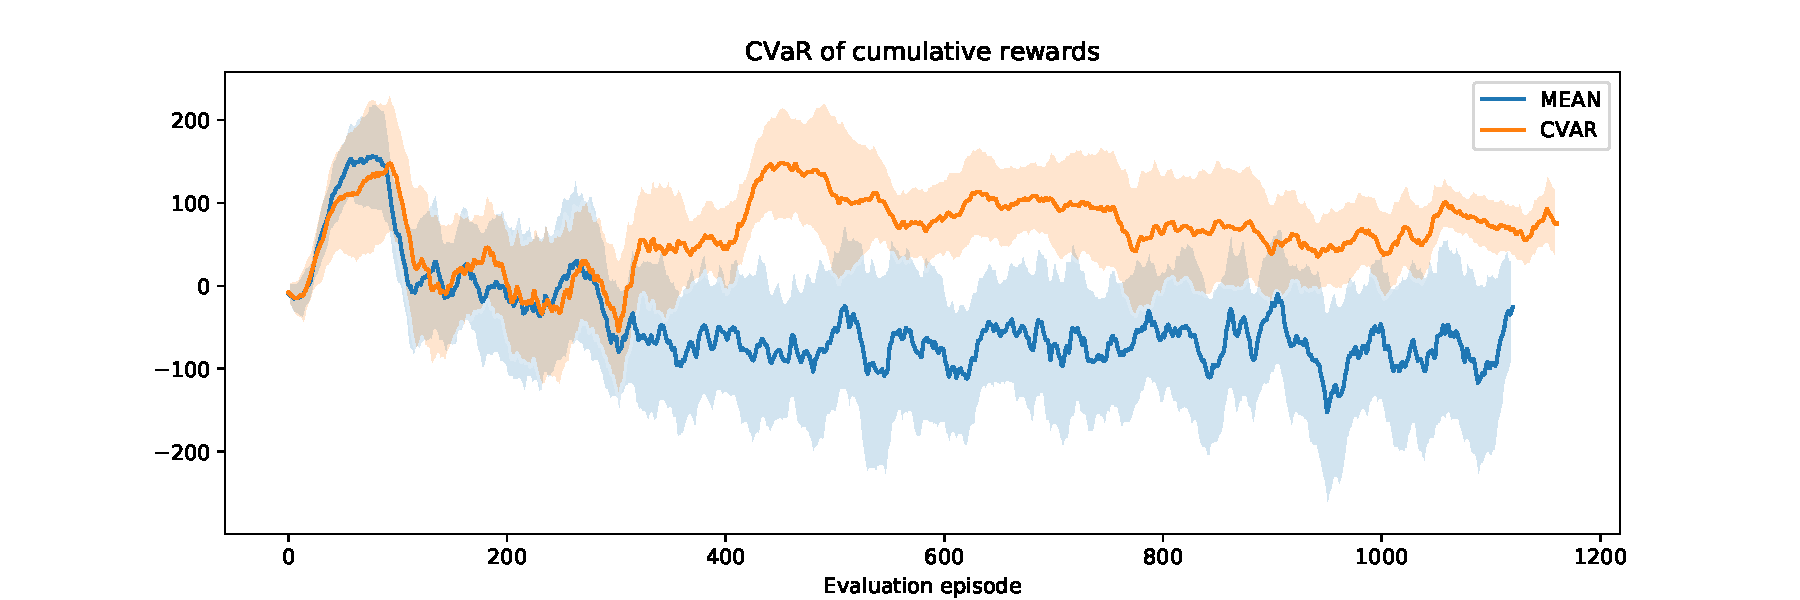
\includegraphics[width=0.8\textwidth]{images/Cheetah_offpolicy_medium/cvar_train_withstds.pdf}
        \caption{CVaR$_\alpha=0.1$ of the cumulative rewards over 5 evaluation episodes.
        Every point corresponds to one evaluation process performed every 1000 steps of training.For the plot we
        show averaged values over 5 random seeds and 1 std}
        \label{fig:cvar_cheetah}
    
\end{figure}

\begin{figure}[ht]
    \centering
    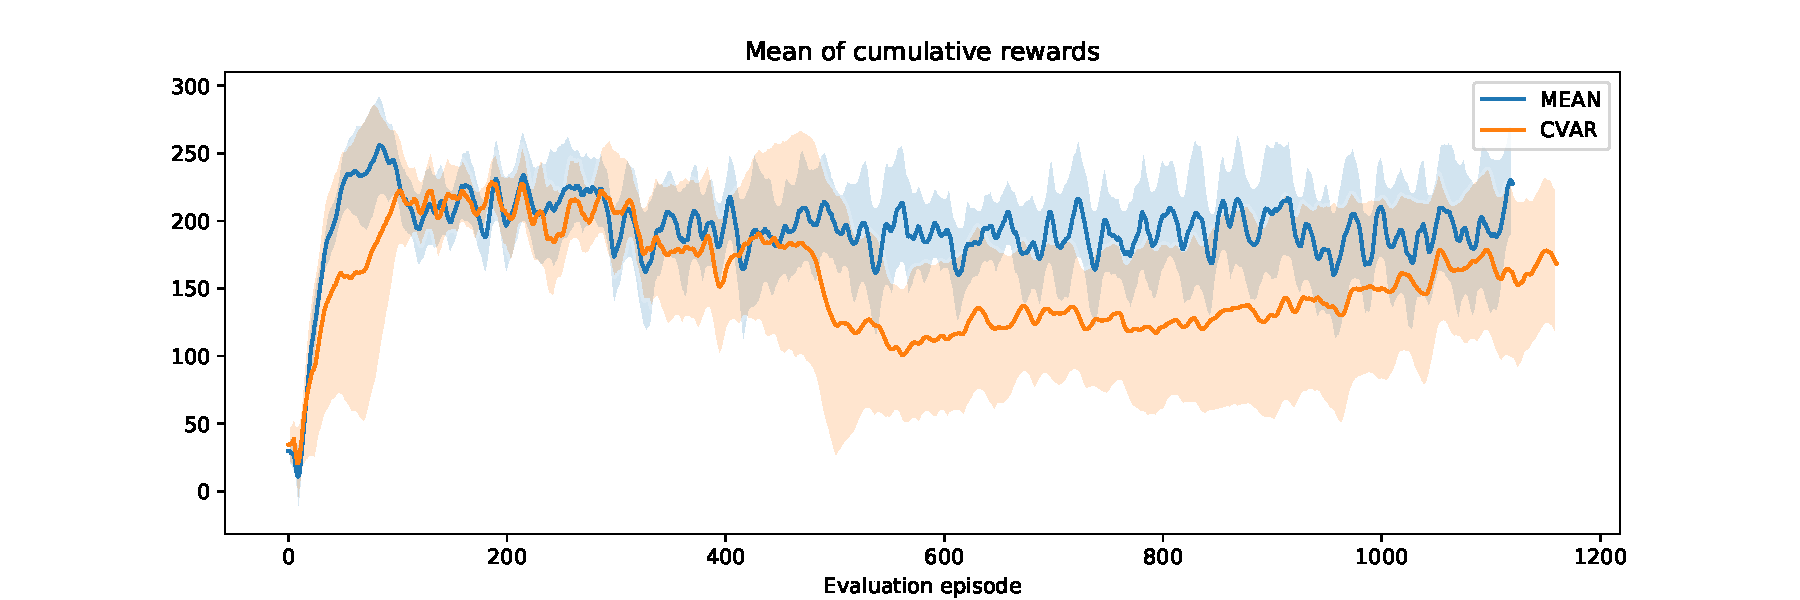
\includegraphics[width=0.8\textwidth]{images/Cheetah_offpolicy_medium/mean_train_withstds.pdf}
    \caption{Mean of the cumulative rewards over 5 evaluation episodes. Every point corresponds
    to one evaluation process performed every 1000 steps of training.For the plot we
    show averaged values over 5 random seeds and 1 std}
    \label{fig:mean_cheetah}

\end{figure}



\begin{figure}[ht]
    \centering
    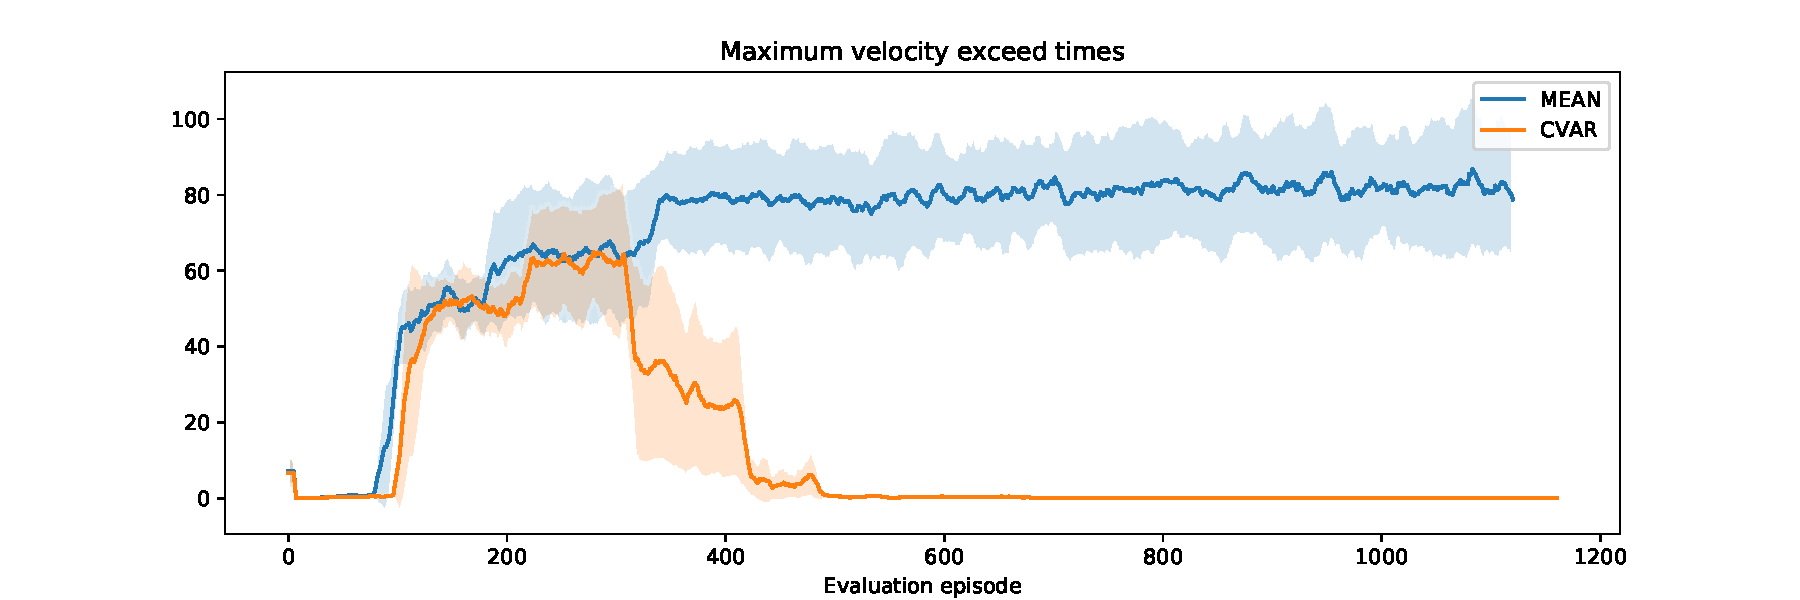
\includegraphics[width=0.8\textwidth]{images/Cheetah_offpolicy_medium/times_exceedvel_withstds.pdf}
    \caption{Mean of number of times the maximum velocity was exceeded over 5 evaluation episodes.
    Every point corresponds to one evaluation process performed every 1000 steps of training.
    For the plot we show averaged values over 5 random seeds and 1 std}
    \label{fig:vel_exceed_cheetah}

\end{figure}

\begin{figure}[ht]
    \centering
    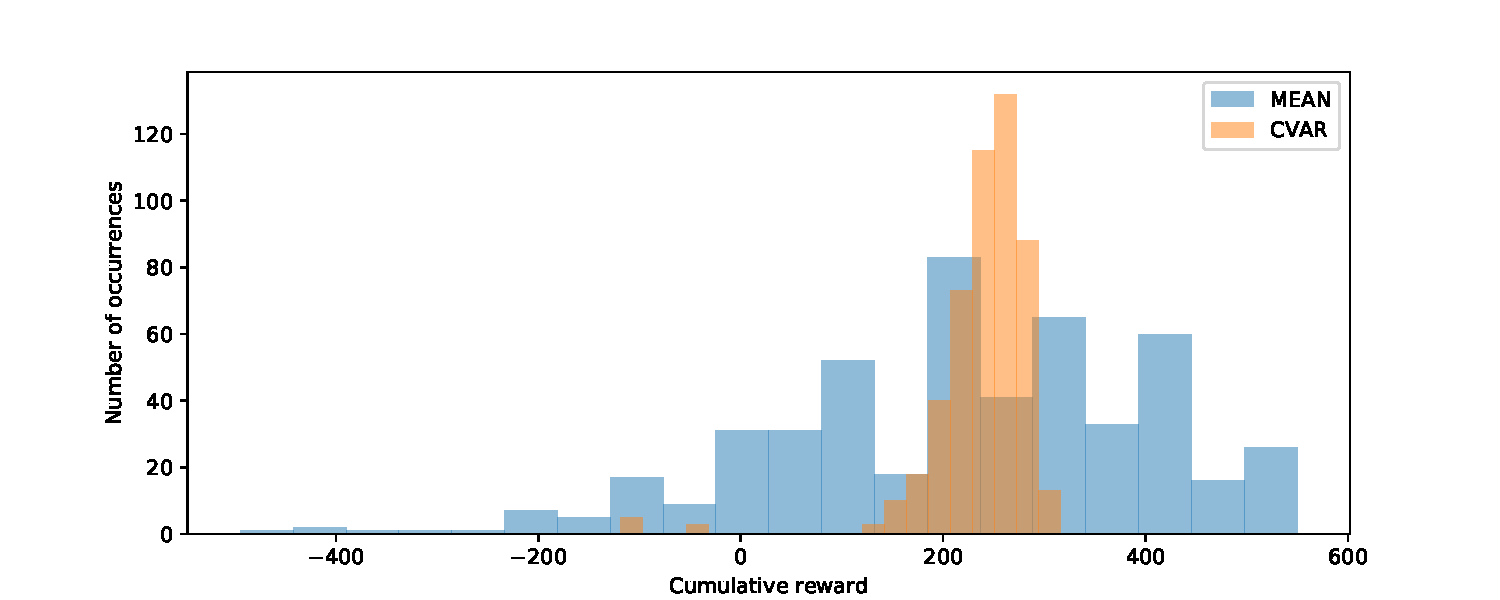
\includegraphics[width=0.8\textwidth]{images/Cheetah_offpolicy_medium/hist_evaluation_numevalsteps200_500eps.pdf}
    \caption{Comparison of cumulative rewards achieved with \textit{CVaR} and \textit{Mean}
    over 500 evaluation episodes of 200 time steps each using the trained final policies.
    \textit{Mean} achieves an expected value  ($\mu=220.75)$  but 
    has a far lower CVAR ($\text{CVaR}_{\alpha= 0.1}$=-131.77) compared to
    \textit{CVaR} ($\mu=238.18$ and $\text{CVaR}_{\alpha= 0.1}$=130.63)}
    \label{fig:hist_cum_rewards200steps_cheetah}
\end{figure}

\clearpage

\subsection{Walker}

We show results on the \textit{Walker2d} task.
In the \textit{Walker2d} environment, a two-dimensional bipedal robot needs to learn walk forward
as fast as possible.
The observation space has 17 dimensions (accounting for velocity and position of the joints)
The control space has a dimensionality of 6, constrained between -1 and 1, 
controlling the torques applied to the joints.
The reward received per step is a function of the control cost, the velocity of the agent and 
and an additional reward per every step for which the agents keep in a \textit{healthy} position.
A \textit{healthy} position is considered when the agent has an angle inclination and center of mass
position constrained between some pre-defined values. Whenever this doesn't hold, the episode ends.

\subsubsection{Dataset}
We use the \textit{walker2d-expert-v0} dataset from D4RL, which consists of 1M samples of data generated by
training to completion a policy online using a standard RL algorithm (soft actor-critic).

The environment is again deterministic, so to proof the performance of our algorithm, we modify the environment to
add a source of uncertainty. We introduce stochasticity in the original cost function in a way that 
makes the environment stochastic enough to have a meaningful assessment of risk in terms of 
tail performance.
In this case, a \textit{robust healthy} range is defined, defining a more constrained subset of the \textit{healthy} range.
A reward of $R_H=-100$ is given with probability 0.1, if the walker exits the \textit{robust healthy} space.

Due to the fact that there is no direct access to the required information from the observations,
we reran the environment interactions from the dataset in open-loop, to collect the desired information and 
modify the rewards accordingly.
The modified dataset was used to train the algorithm in an offline way.

In the following we show the evaluation during training for both \textit{Mean} and
\textit{CVaR}.
Evaluation process is the same as for the cheetah environment.

After training, we used the final policies and deployed them in the noisy environment for 500 episodes 
1000 time steps each. An histogram of the resulting cumulative rewards is added below showing
how the \textit{Mean} algorithm obtain in average higher rewards, but in some scenarios it 
obtains really low results, whereas the \textit{CVaR} performs in average worse than \textit{Mean} 
but the conditional value at risk is higher than for the \textit{Mean}.
Results are shown below.


\begin{figure}[ht]
    \centering
    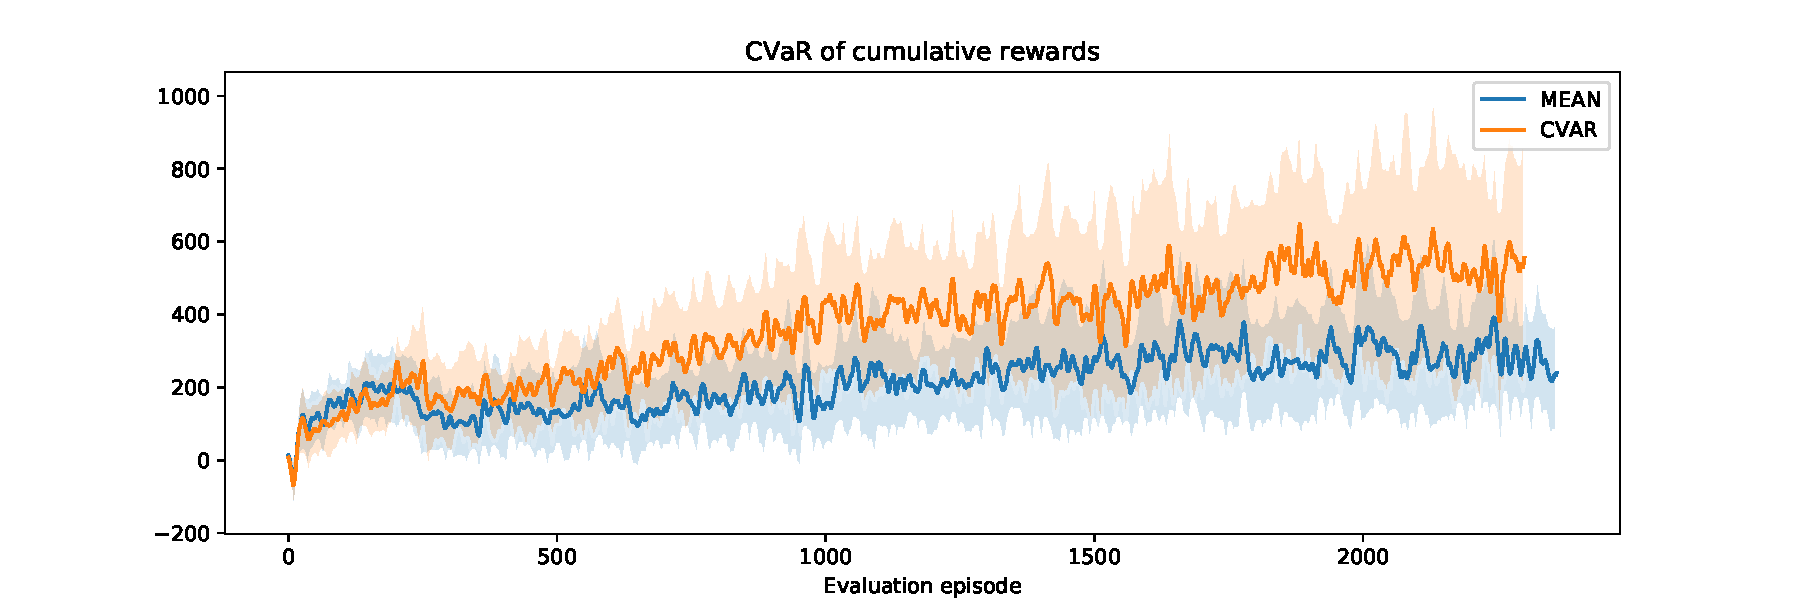
\includegraphics[width=0.8\textwidth]{images/Walker_offpolicy_expert/cvar_train_withstds.pdf}
    \caption{CVaR$_\alpha=0.1$ of the cumulative rewards over 5 evaluation episodes.
    Every point corresponds to one evaluation process performed every 1000 steps of training.For the plot we
    show averaged values over 10 random seeds and 1 std}
    \label{fig:cvar_walker}

\end{figure}

\begin{figure}[ht]
\centering
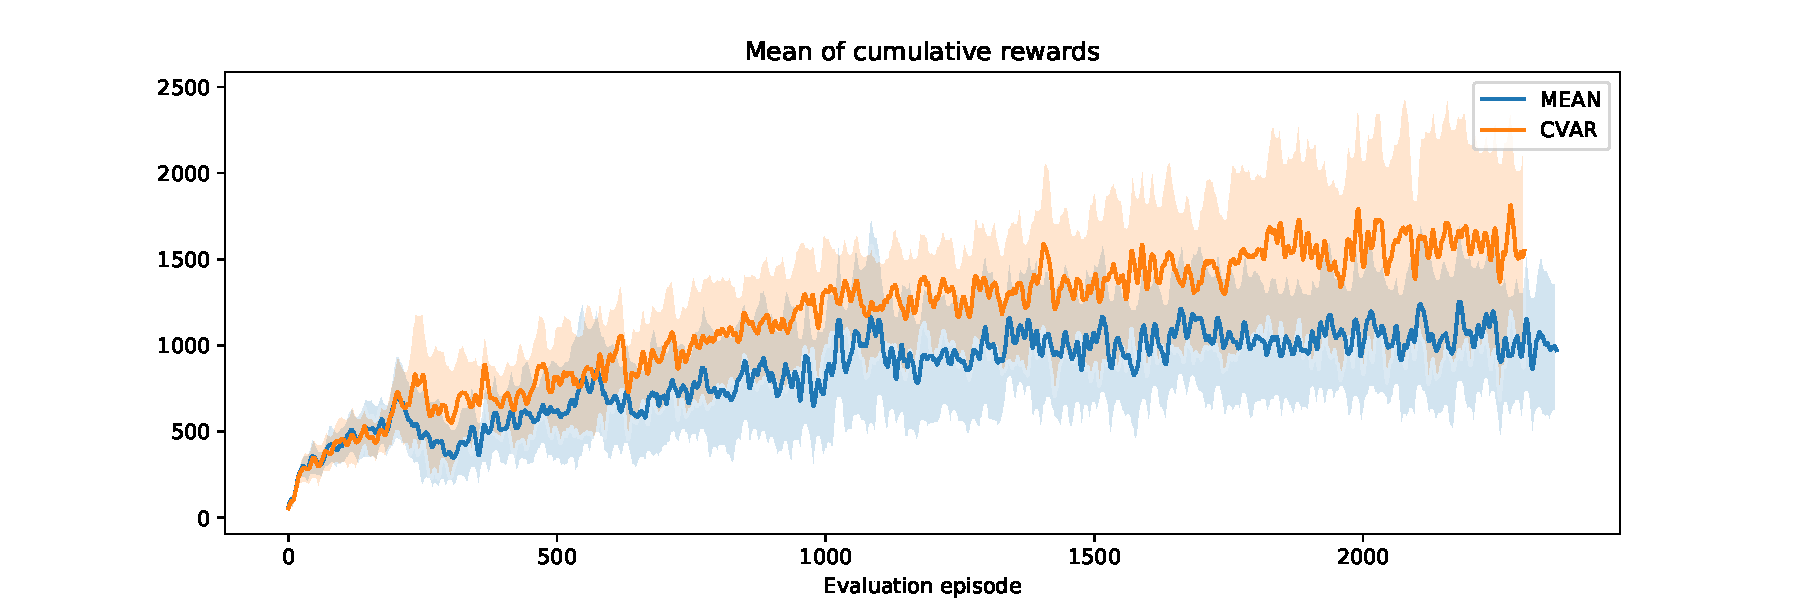
\includegraphics[width=0.8\textwidth]{images/Walker_offpolicy_expert/mean_train_withstds.pdf}
\caption{Mean of the cumulative rewards over 5 evaluation episodes. Every point corresponds
to one evaluation process performed every 1000 steps of training.For the plot we
show averaged values over 10 random seeds and 1 std}
\label{fig:mean_walker}

\end{figure}



\begin{figure}[ht]
\centering
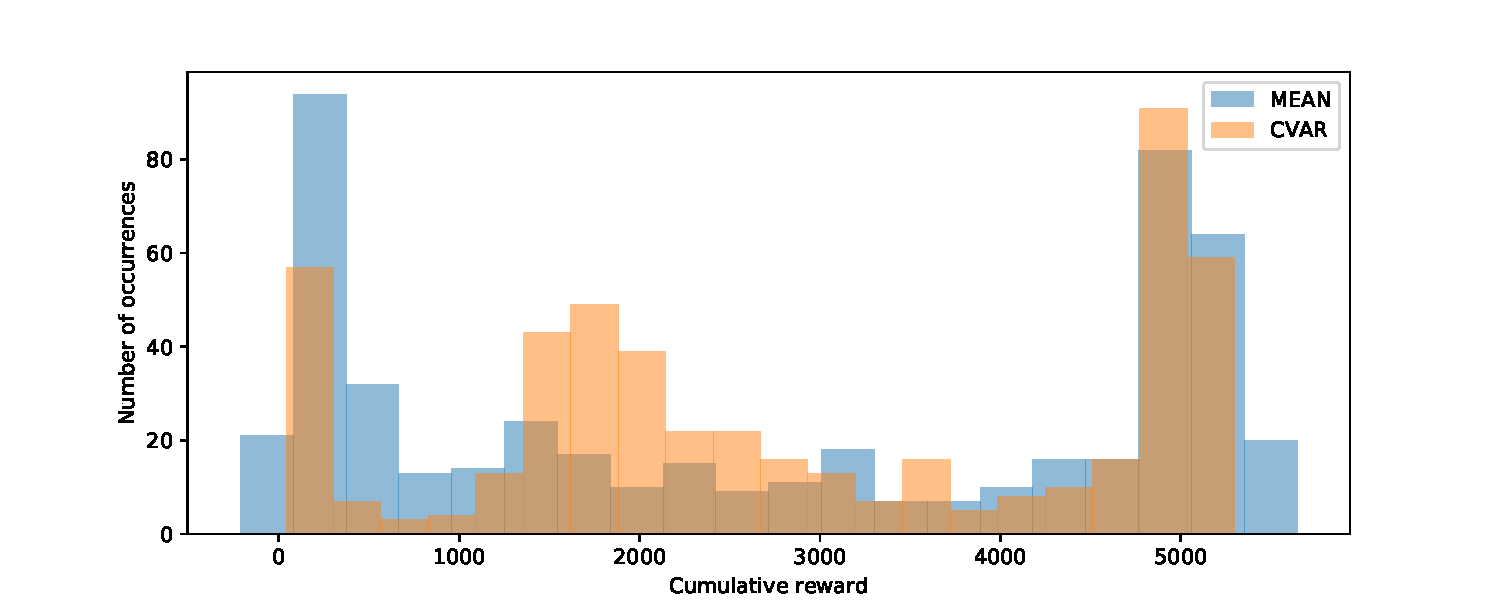
\includegraphics[width=0.8\textwidth]{images/Walker_offpolicy_expert/hist_evaluation_numevalsteps1000.pdf}
\caption{Comparison of cumulative rewards achieved with \textit{CVaR} and \textit{Mean}
over 500 evaluation episodes of 1000 time steps each using the trained final policies.
\textit{Mean} achieves a slightly lower expected value ($\mu=2739.47)$ but 
has a lower CVAR ($\text{CVaR}_{\alpha= 0.1}$=67.54) compared to
\textit{CVaR} ($\mu=2922.56$ and $\text{CVaR}_{\alpha= 0.1}$=235.74)}
\label{fig:hist_cum_rewards_walker}
\end{figure}

\clearpage
\subsection{Medical environment}
Add more environments. To be decided